\chapter{Разработка онтологических моделей} \label{chapt2}

\section{Модель взаимодействия объектов системы дистанционного обучения} \label{sect2_1}

Данные в системе дистанционного обучения ECOLE хранятся в формате RDF(Resource Description Framework). Для хранения данных в системе был разработан набор онтологий. Модель данных системы делится на три основных уровня: уровень предметных областей, уровень учебных материалов, уровень деятельности пользователей в системе. Уровни модели связаны друг с другом для обеспечения взаимодействия различных ресурсов системы. Модель данных представлена на рисунке \ref{img:overall_model}.

\begin{figure} [h] 
  \center
  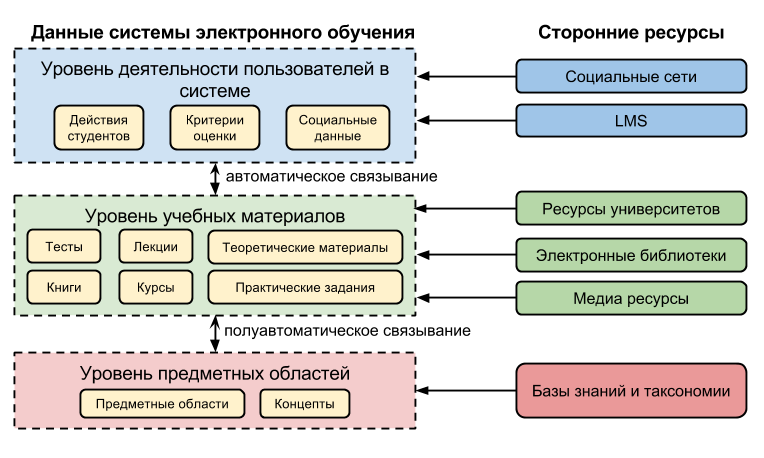
\includegraphics [scale=0.5] {overall_model}
  \caption{Общая модель данных системы дистанционного обучения ECOLE.} 
  \label{img:overall_model}  
\end{figure}

Уровень предметных областей является основой модели данных и содержит информацию о предметных областях науки и образования. Сбор данных для этого уровня производится из сторонних баз знаний, таксономий и опубликованных наборов данных таких как DBpedia и Mathematics Subject Classification. 

Уровень учебных материалов содержит информацию необходимую для проведения учебного процесса. Уровень содержит данные по образовательным программам, курсам, тестам и медиа ресурсам. Сбор данных для этого уровня производится из хранилищ университетов, открытых электронных библиотек и медиа ресурсов. Связывание учебных материалов с предметными терминами и областями производится в полуавтоматическом режим с использованием алгоритмов обработки естественного языка. 

Уровень деятельности пользователей в системе содержит результаты обучения студентов и  статистические данные по активности пользователей. Статистика ведется в системе управления обучением LMS(Learning Management System). При ведении статистики используется информация из социальных сетей. Связывание статистики и результатов обучения с учебными материалами происходит в автоматическом режиме алгоритмами LMS.




\section{Онтология учебных материалов} \label{sect2_2}

Онтология учебных материалов описывает отношения между курсами, модулями, лекциями, тестами, практиками и предметными терминами. Онтология основана на  «врехнеуровневых» онтологиях рекомендованных к использованию при описании учебных материалов.

The Academic Institution Internal Structure Ontology (AIISO) является онтологией описывающей внутреннюю организационную структуру образовательного процесса. AIISO предоставляет классы и свойства для описания курсов и модулей.

The Bibliographic Ontology(BIBO) является онтологией описывающей библиографические ресурсы. В онтологии учебных материалов BIBO используется для описания рекомендованной литературы, научных публикаций, методичек и монографий. 

The Ontology for Media Resources(MA-ONT) является онтологией описывающей медиа ресурсы. С помощью классов и свойств MA-ONT в онтологии учебных материалов производится связывание лекций с видео материалами.

Основными классами онтологии учебных материалов являются: Курс, Модуль, Лекция, Тест, Экзамен, Практика, Предметная область, Предметный термин и Ресурс. Онтология состоит из 32 классов, 42 объектных свойств и 13 свойств-значений. Модель онтологии учебных материалов представлена на рисунке \ref{img:ontology_edu}.

\begin{figure} [h] 
  \center
  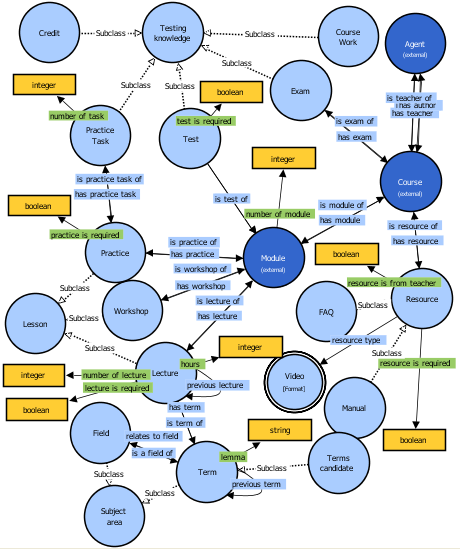
\includegraphics [scale=0.95] {ontology_edu}
  \caption{Основные классы и свойства онтологии учебных материалов.} 
  \label{img:ontology_edu}  
\end{figure}

В основе онтологии учебных материалов лежит модуль предметных терминов и областей. В данном модуле описываются отношения между терминами и объектами онтологии учебных материалов. В модуле описывается ряд вспомогательных классов и свойств для реализации методов гармонизации и анализа данных системы электронного обучения. Модель онтологии предметных терминов и областей представлена на рисунке \ref{img:ontology_term}.  

\begin{figure} [h] 
  \center
  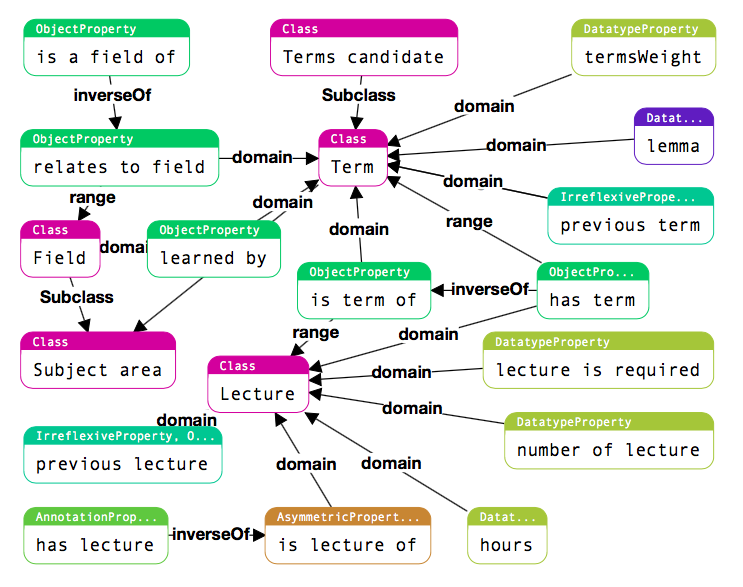
\includegraphics [scale=0.5] {ontology_term}
  \caption{Модель онтологии предметных терминов и областей.} 
  \label{img:ontology_term}  
\end{figure}

Одной из главных особенностей разработанной онтологии является возможность произведения прямого и косвенного междисциплинарного связывания объектов в курсах. Например тест по курсу физики «Интерференция и когерентность» включает в себя использование математических терминов таких как «Вектор» и «Векторное произведение». Если студент не сможет успешно пройти данный тест, система должна рекомендовать к повторению не только лекции по физики, но и определенные лекции по векторной алгебре. Данный пример демонстрирует косвенное связывание курсов физики и векторной алгебры с помощью предметных терминов «Вектор» и «Векторное произведение». Пример представлен на рисунке \ref{img:ontology_edu_example}. Связывание объектов курса с предметными терминами позволяет косвенно связывать лекции, тесты и методические материалы друг с другом.

\begin{figure} [h] 
  \center
  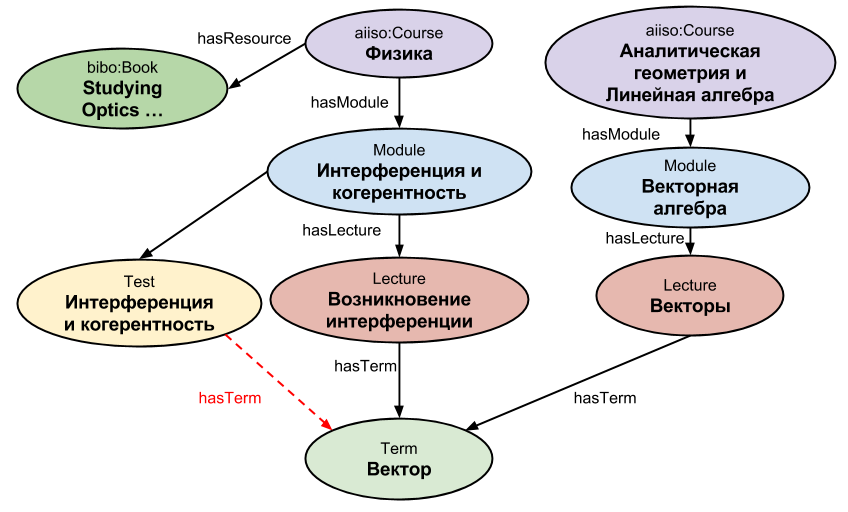
\includegraphics [scale=0.5] {ontology_edu_example}
  \caption{Пример косвенного связывания курсов с помощью предметных терминов.} 
  \label{img:ontology_edu_example}  
\end{figure}




\section{Онтология тестов} \label{sect2_3}

Для описания содержания тестов был разработана онтология тестов. Разработка онтологии производилась методом раскрытия и конкретизации существующих онтологий верхнего уровня. Именно по этому при разработке онтологии использовался нисходящий подход. Онтология тестов содержит классы описывающие тесты, группы и варианты вопросов, задания, ответы, вопросы, различные типы вопросов и ответов. Онтология содержит 12 классов, 10 объектных свойств и 6 свойств-значений. Основной целью онтологии тестов является представление структуры тестов и предоставление возможности автоматического семантического связывания заданий тестов с предметными терминами. Онтология описывает тест как набор из вариантов групп заданий. В каждой группе содержится набор заданий. Задания теста состоят из вопроса и набора ответов. В зависимости от типа вопроса у задания может быть различный набор правильных и неправильных ответов. Связывание предметных терминов с заданиями позволяет описать содержание вопроса и ответов задания.




\section{Онтология активности студента в системе обучения} \label{sect2_4}

Онтология активности студента в системе обучения была разработана для хранения информации о прогрессе и результатах обучения студентов в системе. При разработке были использованы две онтологии верхнего уровня: онтология тестов и онтология Friend Of A Friend (FOAF). Онтология FOAF используется для описания людей и отношений между ними. В дистанционной системе обучения FOAF может быть использована для описания персоналий студентов, преподавателей и других пользователей системы.

Онтология активности студента в системе обучения состоит из 10 классов, 15 объектных свойств и 5 свойств-значений. Основной задачей онтологии является хранение действий студентов в системе. В онтологию может быть записана информация о просмотре студентом видео-лекции, о прохождении теста или завершении курса. Онтология хранит в себе персональные данные студентов. В онтологию включены классы описывающие результаты студентов при прохождении тестов и изучении теоретического материала. Для хранения ответов на тесты конкретного студента используется связывание с онтологией тестов. Связи между студентами, их ответами на задания тестов и предметными терминами позволяют создавать косвенные связи между студентом и объектами курса. На основе полученных косвенных связей возможно реализация персонализированной рекомендательной системы для коррекции процесса обучения студентов. После прохождения теста студент может получить не только оценку, но и список предметных терминов и материалов для повторения составленный на основе ответов на тест.





\section{Онтология оценки знаний студента} \label{sect2_5}

Для реализации методов автоматизированной оценки рейтингов и знаний студентов предметных терминов и областей необходимо разработать и интегрировать в онтологическую модель системы модуль оценки знаний студентов. Модуль оценки знаний студентов - это онтология, которая позволяет хранить вычисленные автоматически оценки знаний студентов по определенным концептам и предметным областям. Онтологическая модель модуля оценки знаний студентов представлена на рисунке \ref{img:ontology_know}.

Онтология модуля содержит класс <<Rate>> (Оценка) и 5 подклассов, которые описывают следующие разновидности оценки:

\begin{itemize}
\item <<Lecture Term Rate>> - оценка предметного термина в контексте лекций; 
\item <<Test Attempt Term Rate>> - оценка предметного термина в контексте прохождения одного теста;
\item <<Average Test Term Rate>> - средняя оценка предметного термина за все тесты;
\item <<Total Term Rate>> - общая оценка предметного термина; 
\item <<Domain Rate>> - оценка предметной области. 
\end{itemize}

Каждый из классов оценки обладает свойством для хранения цифрового значения оценки <<value>>. Также онтология содержит объектные свойства для связывания объектов оценок с объектами студентов из модуля деятельности и результатов студента в системе обучения. В онтологии содержатся объектные свойства для связывания объектов тестов из модуля тестов с объектами терминов из модуля учебных материалов. Разработанная онтология позволяет добавлять новые классы оценок для хранения новых метрик при изменении алгоритмов расчета оценок.

\begin{figure} [h] 
  \center
  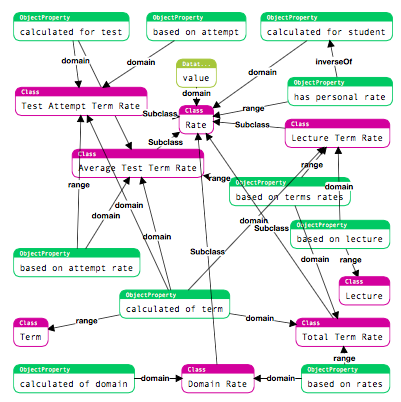
\includegraphics [scale=0.9] {ontology_know}
\caption{Онтологическая модель оценки знаний студентов.}
  \label{img:ontology_know}  
\end{figure}
